%*****************************************
\chapter{Grundlagen}\label{ch:preliminaries}
%*****************************************




\section*{Inhalte des Kapitels}
- Taxonomie von Ammus (\citet{ammus}) % DONE
- Transformer Architektur (\citet{attention}) % DONE

- Neuronales Netz (https://katalog.ub.uni-leipzig.de/Record/0-1066754535) % DONE
- Activation Functions (https://katalog.ub.uni-leipzig.de/Record/0-1066754535) % DONE
- Backpropagation (https://katalog.ub.uni-leipzig.de/Record/0-1066754535)% DONE
- Training eines Modells % DONE
    - Batching % DONE
    - Optimizer % DONE
    - Learning Rate % DONE

- Feed-Forward Netze
- Multi-Head Attention
- Encoder und Decoder

- Input embeddings = Embeddings
- Positional Embeddings
- Tokenization % DONE
    - Byte Pair Encoding % DONE


Sprachmodell Definition (Was ist das)

- Autoregressive Modelle
    - Self-supervised Learning % DONE
    - Pretraining
    - continual Pretraining
    - Decoder-Based
    - ZeroShot / FewShot

- Weiterentwicklungen
    - Deep Residual Connections % DONE
    - DropOut   % DONE

Wissen, Information, Daten (Winter)
FScore, Precision, Recall, Micro und MacroF1 (QUALD9)
Question Answering (Aggregation, erst FScore für Frage, dann Durchschnitt, oder andersrum)
API, Overfitting

\section{Neuronale Netzwerke}
Zum Verständnis der Transformer-Architektur ist es notwendig, die Grundlagen von Neuronalen Netzen zu verstehen.
Neuronale Netze wurden erstmalig 1943 von \citet{neuronal_networks_first} beschrieben und unterliefen seitdem vielen Veränderungen und Verbesserungen.
Eine Beschreibung grundlegender Techniken findet sich in \citet{neuronale-netze}. Auf Basis dieses Buches wird in Folgendem ein Überblick über die Funktionsweise von Neuronalen Netzen gegeben.\\

\subsection{Architektur eines einfachen Neuronalen Netzes}
Neuronale Netze imitieren die Funktionsweise des menschlichen Gehirns mit Hilfe von mathematischen Gleichungen.
Ein Netz besteht aus einer Anzahl an Neuronen, welche sowohl Eingangs- als auch Ausgangsverbindungen zu anderen Neuronen besitzen.
Neuronen besitzen die Eigenschaft, aus gegebenen Eingängen einen Impuls zu den Ausgängen zu senden, wenn ein Schwellwert überschritten ist.
Anders als im Gehirn sind normale Neuronale Netze jedoch logischer aufgebaut.
Neuronen sind in Schichten angeordnet, wobei die erste Schicht die Eingabeschicht bestehend aus Eingabeneuronen $E_N$ und die letzte Schicht die Ausgabeschicht bestehend aus Ausgabeneuronen $A_N$ ist.
Schichten zwischen diesen beiden Grenzen nennt man Hidden Layers mit Neuronen $H^L_N$.\\


\begin{figure}
    \centering
    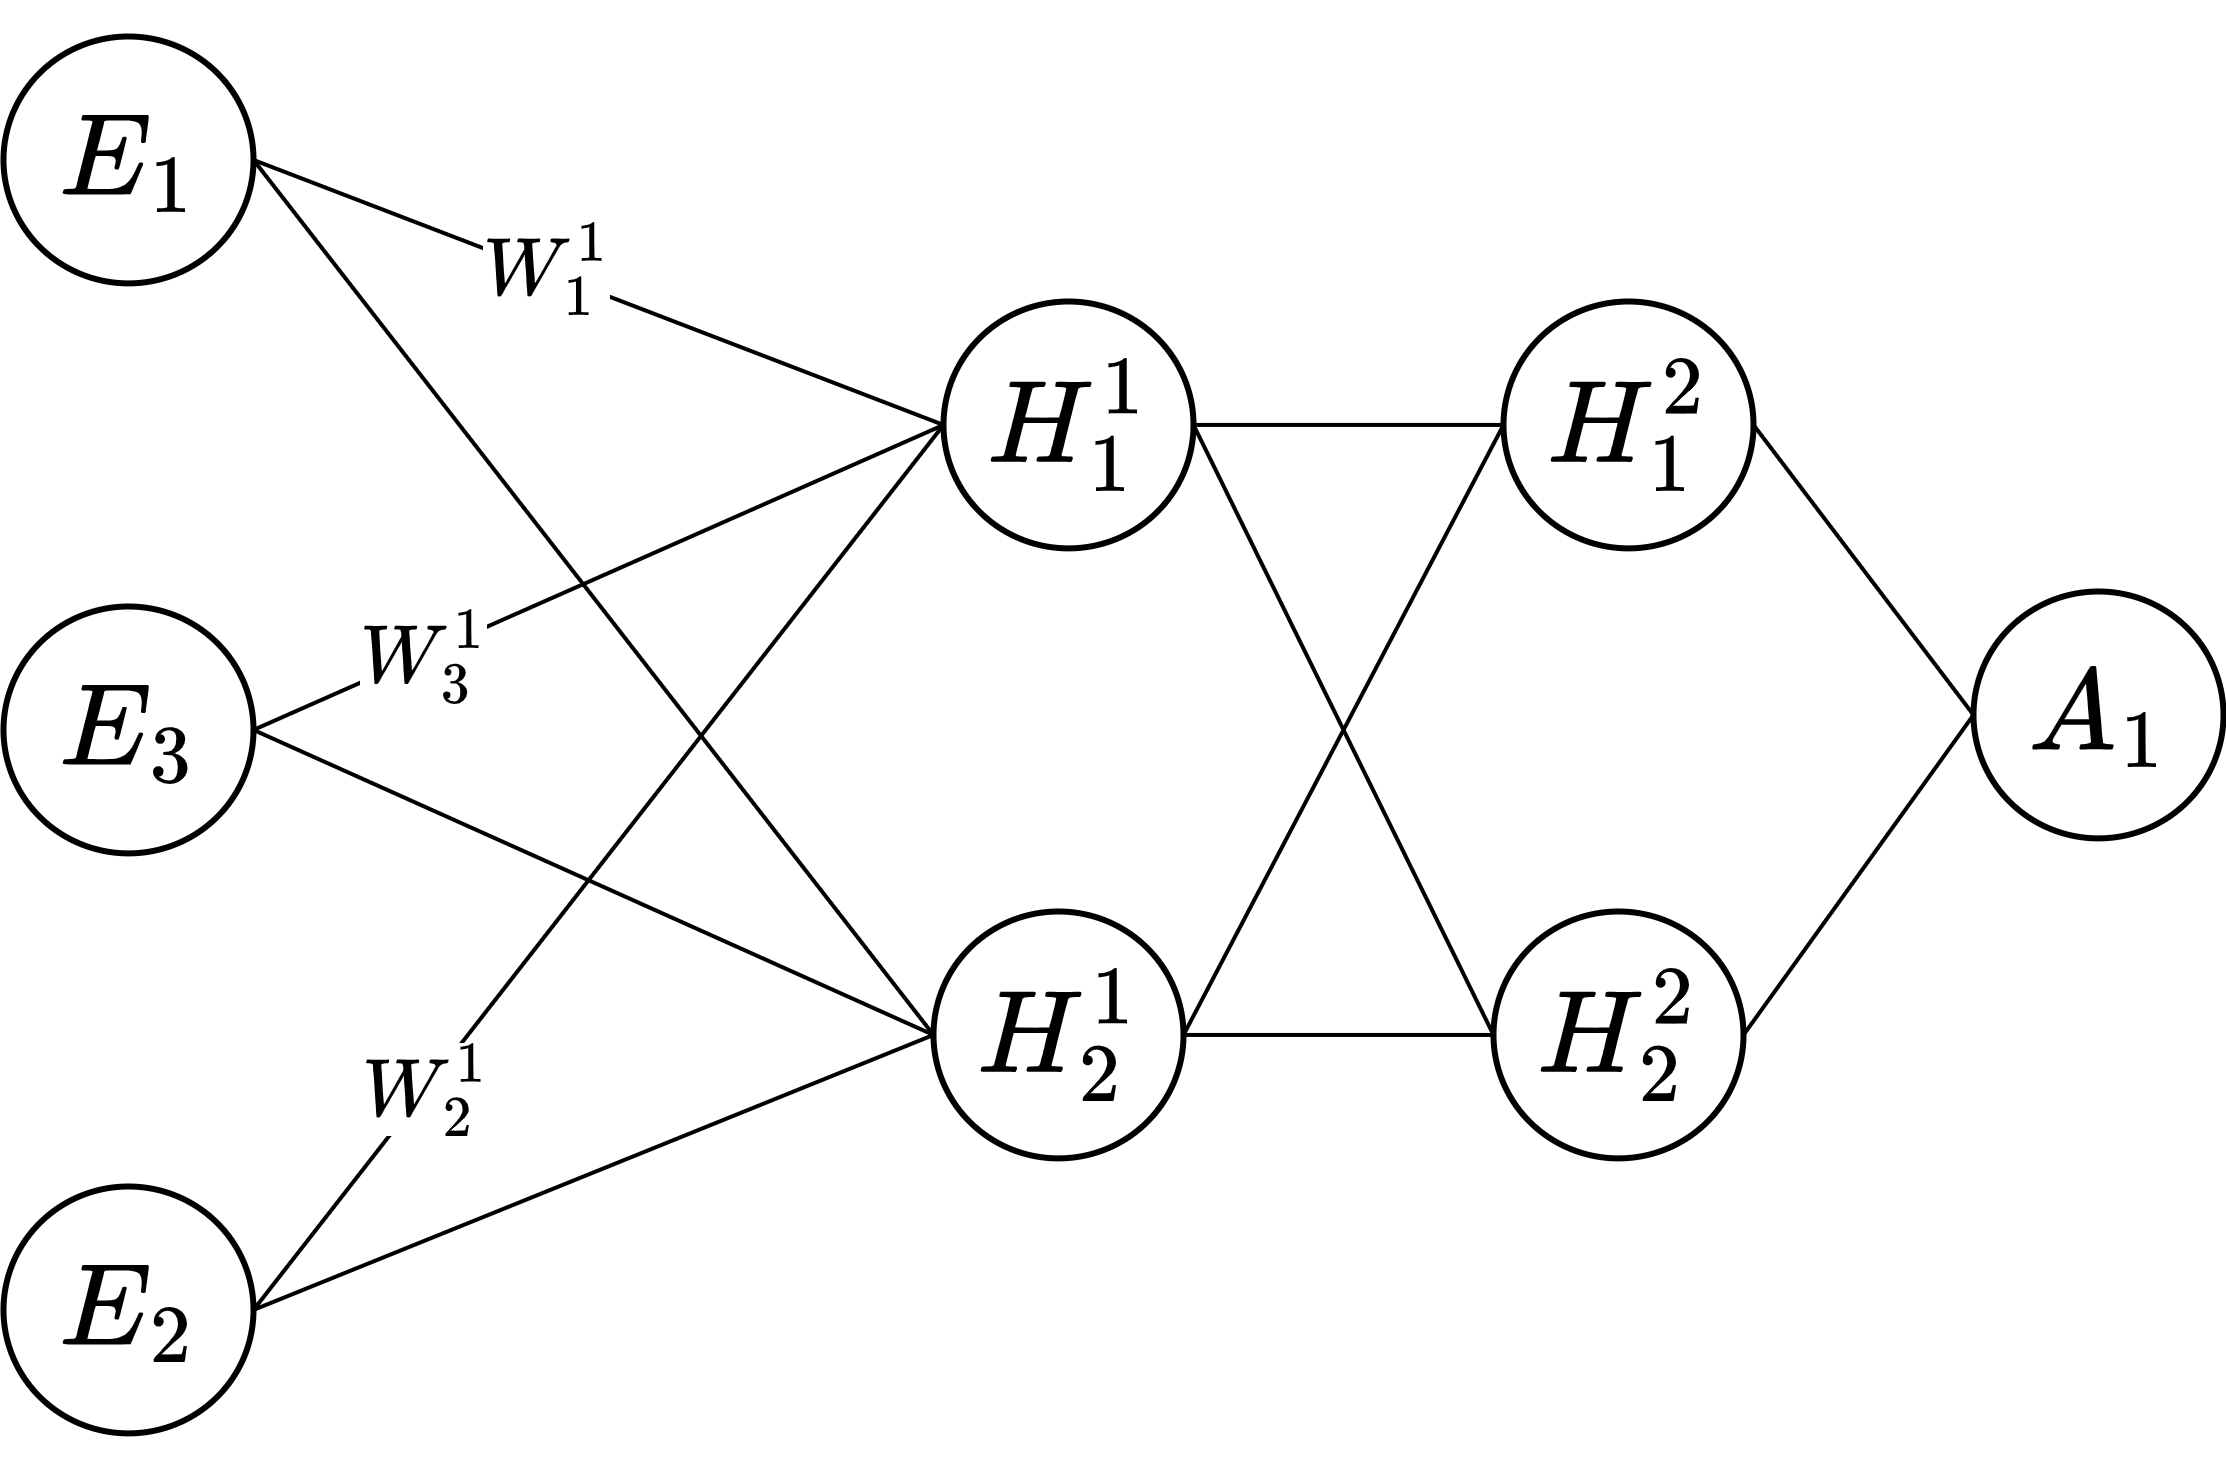
\includegraphics[width=\textwidth]{zeichnungen/nn.png}
    \caption{Beispiel-Aufbau eines Neuronalen Netzes mit 3 Eingabeneuronen, 4 Hidden Neuronen und einem Ausgabeneuron.}\label{nn_simple}
\end{figure}

\cref{nn_simple} zeigt einen Beispielaufbau mit 3 $E_N$, hier bezeichnet als $E_1,E_2,E_3$, zwei Hidden Layer mit je zwei $H_N$, hier bezeichnet als $H^1_1, H^1_2$ und $H^2_1, H^2_2$ und einem Ausgabeneuron $A_1$.
Verbunden sind Neuronen mit sogenannten Gewichten $W_N$. Man spricht hier von einer Vorwärts-Verbindung.
Dies bedeutet das Eingaben durch die Schichten in Richtung der Ausgabe weitergeben werden, jedoch nicht zurück zur Eingabe fließen können.
Im Beispiel in \cref{nn_simple} sind diese Verbindungen vollständig.
Jedes Neuron einer Schicht hat eine Verbindung zu jedem Neuron der nächsten Schicht.
Hier nicht gezeigt enthält jedes Neuron auch eine Eingangsverbindung von einem Bias $B_N$.

\subsection{Funktionsweise eines einfachen Neuronalen Netzes}
Die Nutzung des Neuronalen Netzes erfolgt in zwei Schritten.
Zu erst wird eine Eingabe in die Eingangsneuronen $E_N$ gegeben.
Diese Eingabe wird durch die Schichten weitergegeben, bis sie in der Ausgabeschicht $A_N$ ankommt.
Nun muss das Ergebnis interpretiert werden.\\

Eine Beispielanwendung wäre hier die Erkennung von handgeschriebenen Ziffern.
Die Eingabe wäre hier ein Bild der Ziffer, welches in ein Neuronales Netz gegeben wird.
Jedes Neuron repräsentiert den Grauwert eines Pixels im Bereich $[0,1]$.
Die Ausgabe repräsentiert die erkannte Ziffer.
Für jede mögliche Ziffer (0-9) existiert ein Ausgabeneuron und erhält einen Wert zwischen 0 und 1 durch das Neuronale Netz.
Das Neuron mit der höchsten Ausgabe repräsentiert die erkannte Ziffer.\\

Eine Beispielrechnung für das erste Neuron der ersten Hidden Layer $H^1_1$ ist wie folgt:
\begin{equation}
    H^1_1=ReLU(W^1_1*E_1 + W^1_2*E_2 + W^1_3*E_3 + B^1_1)
\end{equation}
$W^1_N$ repräsentieren hier Gewichte der ersten Schicht.
Gewichte sind Parameter, die während des Trainings eines Netzwerkes angepasst werden, um eine optimale Ausgabe von $A_N$ zu erhalten.
Diese Parameter nennt man auch lernbare Parameter.
$B^1_N$ ist der Bias und ist ebenso ein lernbarer Parameter.
Alle Werte der Eingabe werden der Formel folgend zusammengerechnet und mit Hilfe einer Aktivierungsfunktion umgewandelt.
Diese Aktivierungsfunktion war in früheren Netzen die Sigmoid-Funktion \pcref{eq:sigmoid}.
In modernen Netzen und ebenso in Transformer-Modellen wird hier die ReLU Funktion verwendet \pcref{eq:relu}.
\begin{align}
    f(x) &= \frac{1}{1+e^{-x}}\label{eq:sigmoid}\\
    f(x) &= \max(0,x) \label{eq:relu}
\end{align}

\begin{figure}
    \centering
    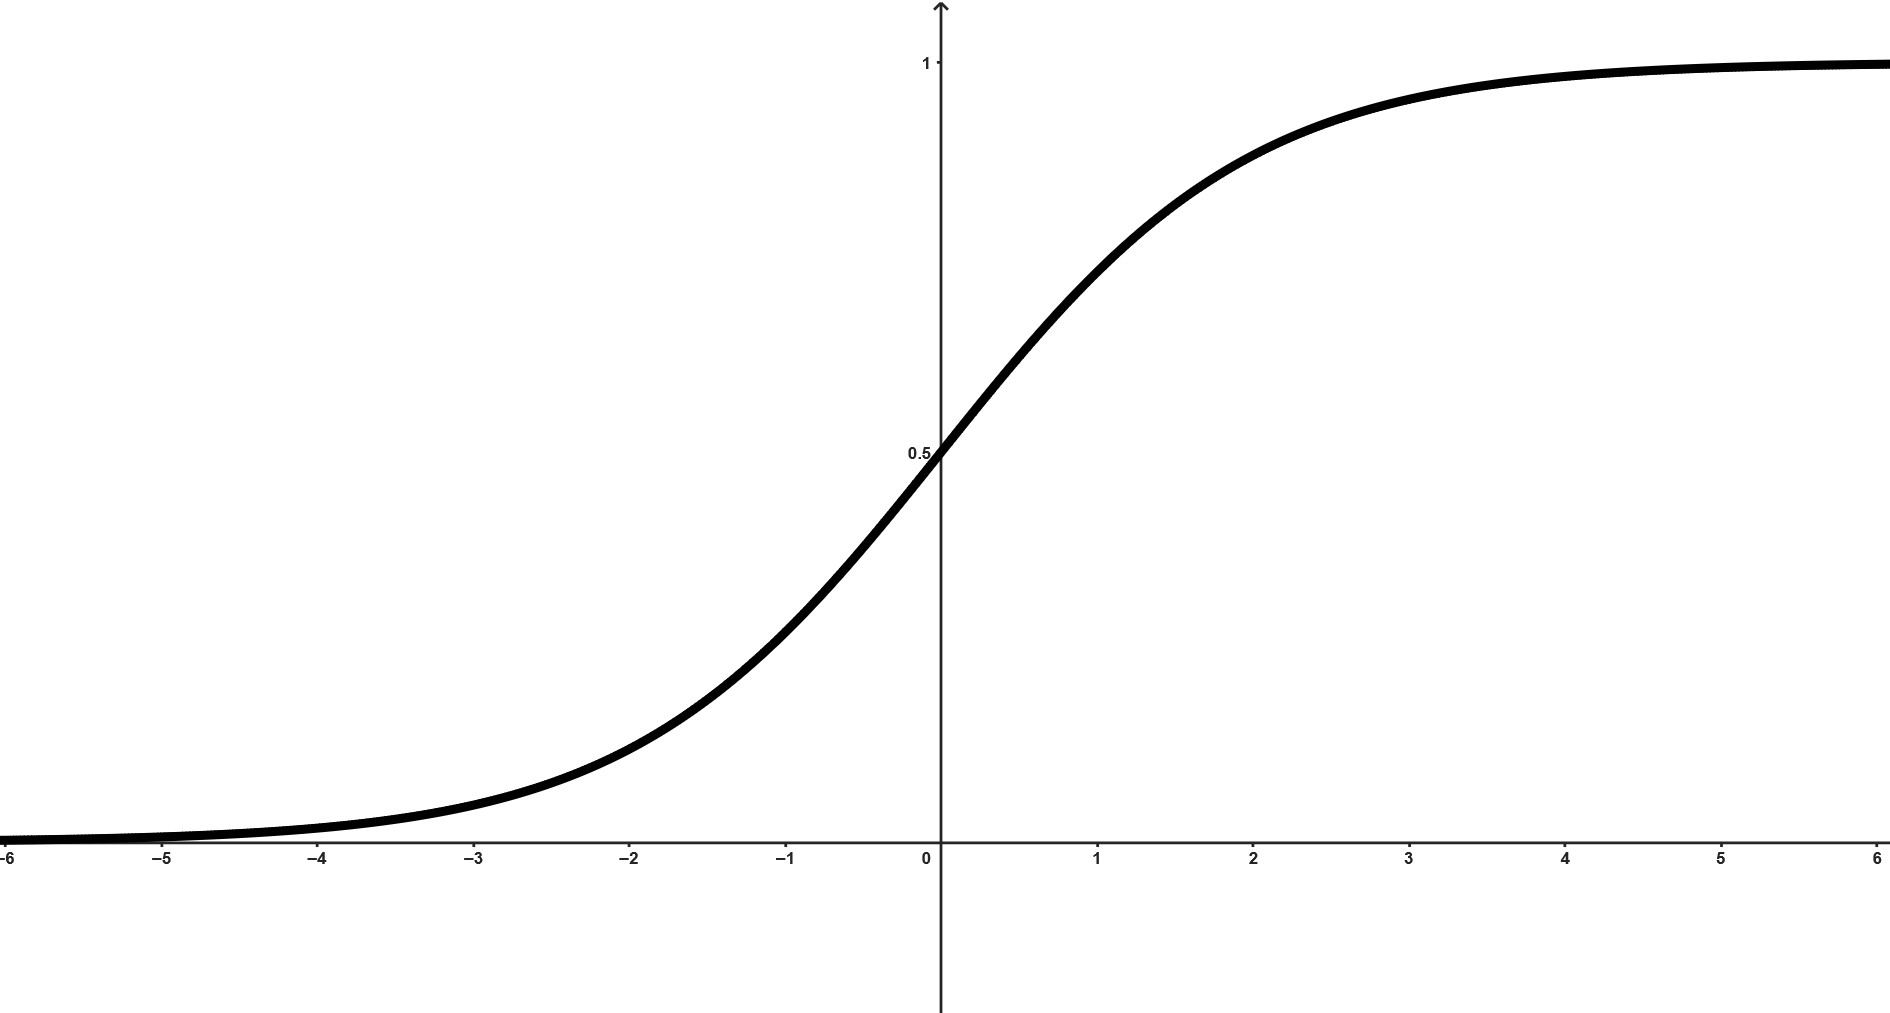
\includegraphics[width=\textwidth]{zeichnungen/sigmoid.png}
    \caption{Die Sigmoid-Funktion}\label{img:sigmoid}
\end{figure}

\begin{figure}
    \centering
    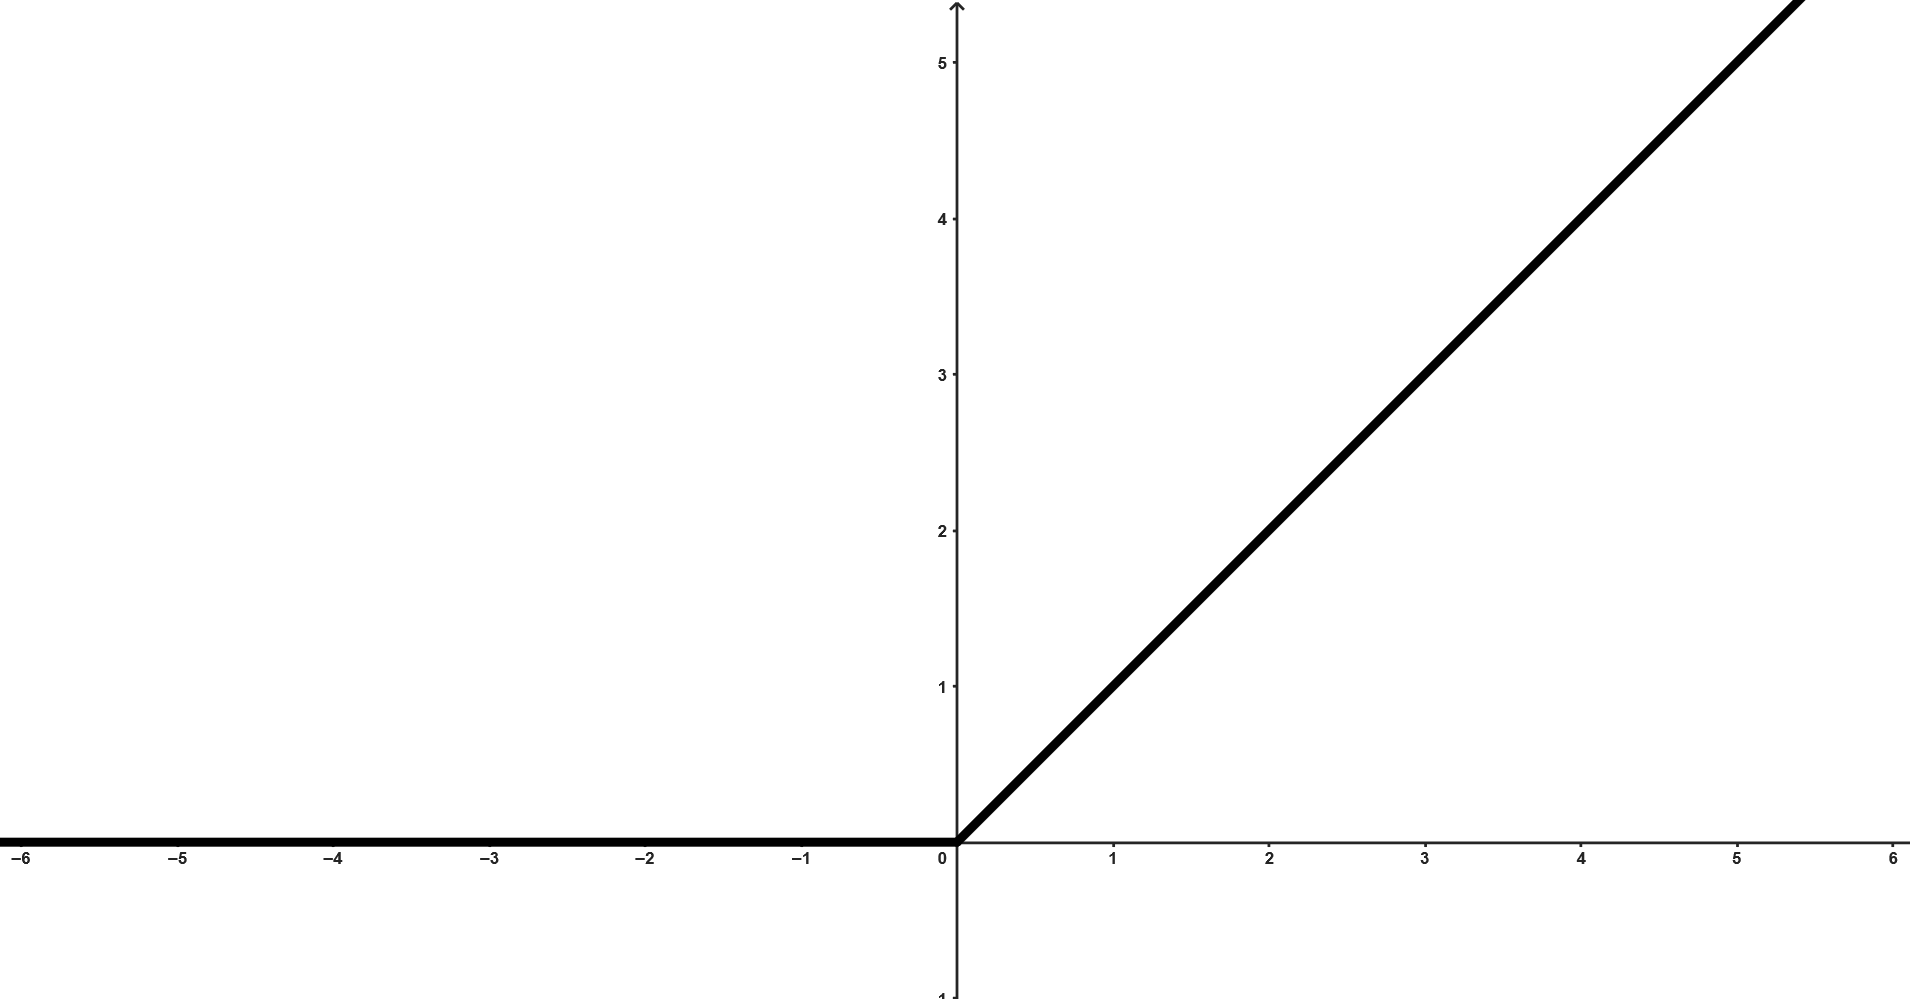
\includegraphics[width=\textwidth]{zeichnungen/relu.png}
    \caption{Die ReLU-Funktion}\label{img:relu}
\end{figure}

Die Funktionen sind in \cref{img:sigmoid,img:relu} dargestellt.
Üblicherweise repräsentiert eine Aktivierungsfunktion eine Transformation der Eingabewerte auf einen nichtlinearen Ausgabewert zwischen 0 und 1.
Jedoch ist dies nicht zwingend notwendig, da zum Beispiel die ReLU Funktion nur Werte zwischen 0 und $\infty$ ausgibt, sich jedoch schneller berechnen lässt als die Sigmoid-Funktion.
Aktivierungsfunktion sind notwendig, um die Komplexität eines Neuronalen Netzes zu erhöhen und damit die Fähigkeit, komplexere Probleme zu lösen, zu ermöglichen.
Ohne eine Aktivierungsfunktion würden $A_N$ Neuronen eine Linearkombination der Eingabewerte ergeben, wodurch hier nur lineare Probleme gelöst werden können.
Ein einfaches Beispiel wäre die Berechnung der XOR-Funktion.
Die XOR-Funktion verbindet zwei Eingaben und ergibt eine Ausgabe. Ist eine der beiden Eingaben 1, soll die Ausgabe ebenso 1 sein.
Andernfalls soll die Ausgabe 0 sein.
Diese einfache Funktion kann nicht ohne eine Aktivierungsfunktion gelöst werden.\\

Die Ausgabe $A_N$ sind ebenso Werte in dem Bereich der Aktivierungsfunktion und sind nicht immer repräsentativ für das Problem, das das Neuronale Netz lösen soll.
Deshalb werden diese Werte interpretiert und repräsentieren häufig einen Confidence-Score für eine bestimmte Klasse.
Ist das Neuron $A_1$ auf dem Maximalwert 1, dann ist das Netz zu \SI{100}{\percent} sicher, dass die Eingabe der Klasse 1 enspricht.
Im Bezug auf Transformer ist die Ausgabe $A_N$ ein Vektor über das gesamte Vokabular des Transformers, und gibt aus, in wie fern das Modell glaubt, das jeweilige Token folgt auf den Eingabetext.\\

\subsection{Training eines Neuronalen Netzes}
Bevor ein Neuronales Netz korrekte Ausgaben liefern kann, muss es trainiert werden.
Trainig bedeutet das iterative Anpassen der lernbaren Parameter, um eine möglichst gute Ausgabe zu erhalten.
Eine gute Ausgabe wird durch eine Fehlerfunktion beschrieben.
Diese Fehlerfunktion gibt einen einzelnen Wert zurück, gegeben der Eingaben in das Neuronale Netz, und steht invers proportional zur richtigen Ausgabe.
Geometrisch repräsentiert eine Fehlerfunktion eine multidimensionale Fläche mit jedem lernbaren Parameter als Achse, in der das Minimum dieser Fläche ein Optimum darstellt.
Dieses Optimum ist das Ziel des Trainings.
Kleine Veränderungen in einzelnen Parametern verändern die Ausgabe der Fehlerfunktion und können somit zeigen, ob diese Veränderung zu einer Verbesserung oder Verschlechterung des Neuronalen Netzes geführt hat.\\

Hier existiert auch bereits die Unterscheidung zwischen einem Überwachten, Selbstüberwachten und Unüberwachten Lernverfahren.
Bei einem Überwachten Lernverfahren sind die gewollten Ausgabeneuronen bekannt und können mit der Ausgabe des Modells verglichen werden.
Dies vereinfacht die Fehlerfunktion, da hier nur die Differenz zwischen den erwarteten Ausgabeneuronen und den tatsächlichen Ausgabeneuronen berechnet werden muss.
Selbstüberwachte Lernverfahren nutzen den selben Prozess, jedoch wird hier die Eingabe genutzt, um die Fehlerfunktion zu berechnen.
Bei Unüberwachtem Lernen ist die Ausgabe nicht bekannt, sondern wird durch einen separaten Prozess interpretiert.\\

Ein Beispiel für ein Überwachtes Lernen wäre die Klassifizierung von Bildern.
Der Datensatz enthält sowohl Bilder, als auch zugehörige Klassen.
Somit ist die erwartete Ausgabe des Modells zu einem Bild exakt die Klasse.
Transformer-Modelle sind Selbstüberwachte Systeme.
Hier ergibt sich aus der Eingabe die Erwartete Ausgabe, da der darauf folgende Token der Eingabe als korrekt angesehen wird.
Unüberwachtes Verfahren sind zum Beispiel Agents, welche Spiele lernen.
Hier existiert in den meisten Fällen eine Belohungsfunktion, welche angibt, wie gut das Modell gespielt hat.
Belohnungsfunktionen können beschreiben, wie weit das Auto im Spiel gefahren ist oder wie viele Punkte gesammelt wurden.\\

\subsubsection{Backpropagation}
Eine der wichtigsten Methoden zum iterativen Anpassen der Gewichte und Bias und damit dem Training von neuronalen Netzen ist die Fehlerrückführungsmethode (engl.
Backprogatation).
Diese Gradienten-Abstiegsmethode wurde erstmalig 1986 von \citet{backpropagation} beschrieben und lässt sich im Detail in \citet{neuronale-netze} nachlesen.
Um den Rahmen dieser Arbeit nicht zu sprengen, wird hier von einer mathematischen Beschreibung abgesehen und nur die Grundidee beschrieben.\\

Die Fehlerfunktion $C$ ist eine Funktion über alle Gewichte und Bias des Neuronalen Netzes und ihrer Ausgabe.
Ihr Minimum zu finden bedeutet ein Optimum für das Modell zu finden.
Zu Beginn des Trainings werden alle Gewichte mit Zufallszahlen initialisiert.
Nun wird die Ausgabe des Modells berechnet und mit der erwarteten Ausgabe verglichen.
Die Funktion $C$ besitzt einen Gradienten $\Delta C$, welcher die Richtung des steilsten Anstiegs der Funktion beschreibt.
Möchte man die Funktion also minimieren, wird der Gradient in die entgegengesetzte Richtung angewandt.
Dieser Gradient setzt sich aus partiellen Ableitung der Fehlerfunktion über alle lernbare Parameter zusammen.\\

\paragraph{Lernrate}
Den Prozess des \enquote{in Richtung des Minimum schreiten} bedeutet, die lernbaren Parameter den partiellen Ableitungen folgend anzupassen.
Die Anpassung der Parameter ist ein Hyperparameter des Trainings und wird als Lernrate bezeichnet (engl. Learning Rate).
Ein Hyperparameter ist ein Parameter, welcher von den Nutzern des Neuronalen Netzes eingestellt wird und nicht erlernt wird.
Wählt man die Lernrate zu hoch, besteht die Gefahr, dass ein Minimum der Fehlerfunktion übersprungen wird und um diesen Punkt osziliert.
Wählt man die Lernrate zu niedrig, braucht das Training des Neuronalen Netzwerkes zu lange um das Minimum zu erreichen.
In Transformern und tiefen Neuronalen Netzen ist die Lernrate nicht konstant, sondern wird über den Prozess des Trainings regelmäßig angpasst.
Sehr große Modelle besitzen oft mehrere Milliarden Parameter und benötigen daher eine sehr kleine Lernrate um nicht zu oszillieren.
Zu Beginn eines Trainings passt sich das Modell mit höhere Lernrate zu stark an kleine Änderungen an und findet ein lokales Minimum, welches weit aus über dem globalen Minimum liegt.
Daher wird eine Aufwärmphase (engl. Warmup) genutzt, um die Lernrate langsam zu erhöhen und das Modell an die Daten anzupassen.
Nach der Aufwärmphase wird die Lernrate langsam verringert, so dass anfänglich große Anpassungen der Parameter möglich sind, gegen Ende des Trainings das gefundene Minimum nur noch feinjustiert wird.\\

\paragraph{Stochastischer Gradientenabstieg}
Die Berechnung des Gradienten der Fehlerfunktion über alle lernbaren Parameter ist nur sinnvoll, wenn sie über den gesamten Datensatz berechnet wird.
Jede Eingabe des Datensatzes verändert die Ausgabe des Modells und somit auch die Fehlerfunktion.
Die Summe der Fehlerfunktionen über alle Eingaben des Datensatzes ist die Fehlerfunktion des gesamten Datensatzes.

\begin{equation}
    C = \frac{1}{n}\sum_{k=0}^{n-1}C_k\\
\end{equation}

Hierbei ist $n$ die Anzahl der Eingaben des Datensatzes und $C_k$ die Fehlerfunktion der $k$-ten Eingabe.
Die Berechnung des Gradienten über alle Eingaben des Datensatzes ist jedoch sehr rechenintensiv und wird daher durch eine Stichprobe des Datensatzes ersetzt.
Diese Stichprobe wird als Batch bezeichnet.
Die Größe des Batches ist ein weiterer Hyperparameter des Trainings.
Die Berechnung des Gradienten über einen Batch wird als Stochastischer Gradientenabstieg (engl.
Stochastic Gradient Descent) bezeichnet, da die Stichprobe des Datensatzes nur eine Approximation des Gradienten ist.
Dadurch gleicht die Richtung des Gradient nur noch annäherungsweise dem tatsächlichen Gradienten, die Berechnung verläuft jedoch deutlich schneller.
Die Größe der Batches ist ein Kompromiss zwischen der Genauigkeit des Gradienten und der Geschwindigkeit der Berechnung.\\

\section{Transformer}\label{sec:transformer}
%\todo{
%Grundlagen:
%- das was du schon drin hast mit "General Pretrained Transformer - Neuronal Networks - Zero Shot Ansatz - Finetuning - Datenkuration"
%- aber alles was mit GPT zu tun hat nicht, das ist ein spezieller Ansatz und das sollte zu state of the art
%- alles was im Titel steht :-) Question Answering, unsupervised und supervised training und so
%- Definitionen Daten, Informationen und Wissen nach Winter passt hier denke ich auch rein
%
%State of the Art:
%- aktuelle Paper
%- Vergleich verschiedener Systeme und Modelle
%- und das was du da schon hast, also das meiste ist ja schon am richtigen Ort
%}
Die erste schriftliche Erwähnung des Transformer-Modells und zusätzlich auch die Einführung der beiden Teilmodelle Encoder und Decoder findet sich in \citet{attention}.
Die hier beschriebene bidirektionale Architektur bildet die Grundlage für alle darauf aufbauenden Modelle und Weiterentwicklungen.
Die grundlegende Architektur wurde für verschiedene Anwendungen stark modifiziert.
Seit 2017 gibt es grundlegende Unterschiede in den Modellen und deren Möglichkeiten.
Aus diesem Grund haben \citet{ammus} eine Taxonomie der Transformer-basierten vortrainierten Sprachmodelle eingeführt.
Diese Taxonomie wird hier zur Beschreibung weiterer Architekturen und Methodiken verwendet.\\

Neben dem Grundbaustein eines Transformers - dem Attention-\ac{nn} - sind zwei wichtige Modifikationen gegenüber normalen neuronalen Netzen in Transformer eingeflossen.
Residuale Verbindungen als Level-Normalisierung, auf Englisch \enquote{Deep Residual Connections}, verändern das Ziel eines \ac{nn}, behalten aber durch ihre Level-Normalisierung die gleichen Ausgaben bei.
Dieses Konzept wurde erstmals in \citet{deep_residual} eingeführt und liefert die Lösung für ein grundlegendes Problem von großen, aus mehreren Ebenen bestehenden Transformer-Modellen.
Bereits 2016 wurde im Bereich der Bilderkennung festgestellt, dass sich die Korrektheit von Modellen mit zunehmender Tiefe sättigt und dann schnell verschlechtert, wenn dieses Modell weiter trainiert wird.
Dies setzte eine praktische Grenze für die Tiefe von \ac{nn}s und verhinderte somit die Lösung komplexerer Probleme mit größeren Modellen.
\citet{deep_residual} beschreiben eine Lösung durch die genannten Residuen, die normale \ac{nn} simple ersetzen können, und zeigen ebenfalls die Wirksamkeit dieser Methode.\\

Die zweite wichtige Änderung ist die Einführung von Dropout.
Dropout ist eine Methode, die die Trainingszeit von \ac{nn}s verkürzt und die Generalisierung verbessert.
\citet{dropout} beschreiben die Methode als das zufällige Aussetzen von Neuronen in einem \ac{nn}. 
Diese Aussetzung hängt nicht von der Eingabe ab.
Durch das Aussetzen von Neuronen wird das \ac{nn} gezwungen, sich nicht auf andere Neuronen zu verlassen und somit eine bessere Generalisierung zu erreichen.
Das Aussetzen erfolgt nur während des Trainings und nicht während der Inferenz.
Die Methode wurde 2014 eingeführt und ist seitdem ein fester Bestandteil von \ac{nn}s.\\

\section{Tokenization}\label{sec:tokenization}
Transformer-Modelle können Eingaben nicht ohne zusätzliche Umwandlung verarbeiten.
Neben der Erzeugung von Kodierungsvektoren muss die Eingabe zunächst in kleinere Einheiten, sogenannte Tokens, zerlegt werden.
Verschiedene ältere Modelle verwenden dazu Wörter oder Symbolunterteilungen.
Dies ist jedoch problematisch.\\

Durch die Zerlegung der Eingaben in Symbole ist zwar das Vokabular kleiner, welches zu schnelleren Trainingsdurchläufen führt, jedoch muss das Modell vor dem Erlernen von Wortzusammenhängen, Satzstrukturen und Sachverhalten zunächst die Bedeutung der Wörter und deren Zusammensetzung aus Symbolen erlernen.
Dies führt dazu, dass ein großer Teil der Trainingszeit für das Erlernen der Sprache verloren geht, was die endgültige Leistungsfähigkeit der Modelle massiv einschränkt \citep{bpe}.
Eine logische Schlussfolgerung wäre hier die Verwendung von Wörtern oder sogar Satzphrasen als Tokens.
Mit zunehmender Größe der Datensätze, die zum Training der Modelle verwendet werden, wächst hier das Vokabular immens an.
Dies führt zu einer starken Verlangsamung der Trainingsläufe und zu sehr großen Modellen ohne Vorteil in ihrer Leistungsfähigkeit.
Wörter mit gleichem Wortstamm oder ähnlicher Bedeutung aufgrund grammatikalischer Regeln (Plural, Genus, Tempora) müssen vom Modell erst als \enquote{gleiches Wort} gelernt werden.
Daher hat sich die Unterteilung von Wörtern in Teilwörter als Standard durchgesetzt.

\subsection{Byte-Pair-Encoding}\label{subsec:bpe}
\citet{bpe} schlugen zu diesem Zweck die Verwendung von \ac{bpe} vor.
Die Unterteilung von Wörtern in Untergruppen von Wörtern hat bereits bei der Übersetzung von Sätzen zu erheblichen Verbesserungen geführt.
Sie hat sich aber auch in anderen Bereichen und Aufgaben wie der Textgenerierung, der Textklassifikation und der Analyse von Emotionen durchgesetzt.
Die Unterteilung von Wörtern ist hier eher als das Zusammenfügen kleinerer Teilwörter zu verstehen.
Ausgehend von einem Vokabular, das aus allen Symbolen eines Alphabets besteht, wird dieses durch das Zusammenführen (engl.
\enquote{Merge}) von Symbolen erweitert, deren Kombination im Datensatz am häufigsten vorkommt.
Dieser Vorgang wird solange wiederholt, bis die gewünschte Anzahl von Teilwörtern erreicht ist.
Die Anzahl der Teilwörter ist dabei ein Hyperparameter, der je nach Modell und Datensatz variiert.\\

Die Unterteilung von Wörtern in Teilwörter hat den Vorteil, dass die Größe des Vokabulars nicht mit der Größe des Datensatzes wächst.
Dies führt zu einer schnelleren Eingabeverarbeitung und einer besseren Generalisierung der Modelle.
Die Unterteilung von Wörtern in Teilwörter hat jedoch auch Nachteile.
Sie ist nicht eindeutig, d.h.
ein Wort kann in unterschiedliche Mengen von Teilwörtern zerlegt werden.
Dies führt zu einer größeren Anzahl möglicher Eingaben, die das Modell lernen muss.
Ein weiterer Nachteil ist, dass die Zerlegung von Wörtern in Teilwörter nicht immer sinnvoll ist.
So kann es vorkommen, dass ein Wort in Teilwörter zerlegt wird, die in der Sprache nicht existieren.
Dies wiederum minimiert die Verallgemeinerbarkeit der Modelle.
Ein Beispiel hierfür ist das Wort \enquote{Datensatz}.
Eine sinnvolle Unterteilung wäre hier \enquote{Daten} und \enquote{satz}, aber durch den Aufbau des Vokabulars aus den Symbolen des Datensatzes kann es vorkommen, dass das Teilwort \enquote{Daten} nicht die notwendige Häufigkeit besitzt und somit nicht im Vokabular vorhanden ist.
Daher muss auch dieses Wort zerlegt werden, z.B.
in \enquote{Da} und \enquote{ten}.
Beide Teilwörter haben in der deutschen Sprache keine Bedeutung, werden aber durch das Modell mit Bedeutung belegt und in Beziehung zu anderen Wörtern gesetzt.
Dies führt zu einer unverständlichen Bedeutungsannotation von Teilwörtern und verschlechtert sowohl die Leistung als auch die Nachvollziehbarkeit des Modells und erschwert die Forschung an den Modellen.


